\documentclass[11pt,ngerman,toc=listof,index=totoc]{scrreprt}
\usepackage{lmodern}
\usepackage{amssymb,amsmath}
\usepackage{ifxetex,ifluatex}
\usepackage{fixltx2e} % provides \textsubscript
\ifnum 0\ifxetex 1\fi\ifluatex 1\fi=0 % if pdftex
  \usepackage[T1]{fontenc}
  \usepackage[utf8]{inputenc}
\else % if luatex or xelatex
  \ifxetex
    \usepackage{mathspec}
  \else
    \usepackage{fontspec}
  \fi
  \defaultfontfeatures{Ligatures=TeX,Scale=MatchLowercase}
\fi
% use upquote if available, for straight quotes in verbatim environments
\IfFileExists{upquote.sty}{\usepackage{upquote}}{}
% use microtype if available
\IfFileExists{microtype.sty}{%
\usepackage{microtype}
\UseMicrotypeSet[protrusion]{basicmath} % disable protrusion for tt fonts
}{}
\usepackage{hyperref}
\hypersetup{unicode=true,
            pdfborder={0 0 0},
            breaklinks=true}
\urlstyle{same}  % don't use monospace font for urls
\ifnum 0\ifxetex 1\fi\ifluatex 1\fi=0 % if pdftex
  \usepackage[shorthands=off,main=ngerman]{babel}
\else
  \usepackage{polyglossia}
  \setmainlanguage[]{german}
\fi
\usepackage{color}
\usepackage{fancyvrb}
\newcommand{\VerbBar}{|}
\newcommand{\VERB}{\Verb[commandchars=\\\{\}]}
\DefineVerbatimEnvironment{Highlighting}{Verbatim}{commandchars=\\\{\}}
% Add ',fontsize=\small' for more characters per line
\newenvironment{Shaded}{}{}
\newcommand{\KeywordTok}[1]{\textcolor[rgb]{0.00,0.44,0.13}{\textbf{{#1}}}}
\newcommand{\DataTypeTok}[1]{\textcolor[rgb]{0.56,0.13,0.00}{{#1}}}
\newcommand{\DecValTok}[1]{\textcolor[rgb]{0.25,0.63,0.44}{{#1}}}
\newcommand{\BaseNTok}[1]{\textcolor[rgb]{0.25,0.63,0.44}{{#1}}}
\newcommand{\FloatTok}[1]{\textcolor[rgb]{0.25,0.63,0.44}{{#1}}}
\newcommand{\ConstantTok}[1]{\textcolor[rgb]{0.53,0.00,0.00}{{#1}}}
\newcommand{\CharTok}[1]{\textcolor[rgb]{0.25,0.44,0.63}{{#1}}}
\newcommand{\SpecialCharTok}[1]{\textcolor[rgb]{0.25,0.44,0.63}{{#1}}}
\newcommand{\StringTok}[1]{\textcolor[rgb]{0.25,0.44,0.63}{{#1}}}
\newcommand{\VerbatimStringTok}[1]{\textcolor[rgb]{0.25,0.44,0.63}{{#1}}}
\newcommand{\SpecialStringTok}[1]{\textcolor[rgb]{0.73,0.40,0.53}{{#1}}}
\newcommand{\ImportTok}[1]{{#1}}
\newcommand{\CommentTok}[1]{\textcolor[rgb]{0.38,0.63,0.69}{\textit{{#1}}}}
\newcommand{\DocumentationTok}[1]{\textcolor[rgb]{0.73,0.13,0.13}{\textit{{#1}}}}
\newcommand{\AnnotationTok}[1]{\textcolor[rgb]{0.38,0.63,0.69}{\textbf{\textit{{#1}}}}}
\newcommand{\CommentVarTok}[1]{\textcolor[rgb]{0.38,0.63,0.69}{\textbf{\textit{{#1}}}}}
\newcommand{\OtherTok}[1]{\textcolor[rgb]{0.00,0.44,0.13}{{#1}}}
\newcommand{\FunctionTok}[1]{\textcolor[rgb]{0.02,0.16,0.49}{{#1}}}
\newcommand{\VariableTok}[1]{\textcolor[rgb]{0.10,0.09,0.49}{{#1}}}
\newcommand{\ControlFlowTok}[1]{\textcolor[rgb]{0.00,0.44,0.13}{\textbf{{#1}}}}
\newcommand{\OperatorTok}[1]{\textcolor[rgb]{0.40,0.40,0.40}{{#1}}}
\newcommand{\BuiltInTok}[1]{{#1}}
\newcommand{\ExtensionTok}[1]{{#1}}
\newcommand{\PreprocessorTok}[1]{\textcolor[rgb]{0.74,0.48,0.00}{{#1}}}
\newcommand{\AttributeTok}[1]{\textcolor[rgb]{0.49,0.56,0.16}{{#1}}}
\newcommand{\RegionMarkerTok}[1]{{#1}}
\newcommand{\InformationTok}[1]{\textcolor[rgb]{0.38,0.63,0.69}{\textbf{\textit{{#1}}}}}
\newcommand{\WarningTok}[1]{\textcolor[rgb]{0.38,0.63,0.69}{\textbf{\textit{{#1}}}}}
\newcommand{\AlertTok}[1]{\textcolor[rgb]{1.00,0.00,0.00}{\textbf{{#1}}}}
\newcommand{\ErrorTok}[1]{\textcolor[rgb]{1.00,0.00,0.00}{\textbf{{#1}}}}
\newcommand{\NormalTok}[1]{{#1}}
\IfFileExists{parskip.sty}{%
\usepackage{parskip}
}{% else
\setlength{\parindent}{0pt}
\setlength{\parskip}{6pt plus 2pt minus 1pt}
}
\setlength{\emergencystretch}{3em}  % prevent overfull lines
\providecommand{\tightlist}{%
  \setlength{\itemsep}{0pt}\setlength{\parskip}{0pt}}
\setcounter{secnumdepth}{5}
% Redefines (sub)paragraphs to behave more like sections
\ifx\paragraph\undefined\else
\let\oldparagraph\paragraph
\renewcommand{\paragraph}[1]{\oldparagraph{#1}\mbox{}}
\fi
\ifx\subparagraph\undefined\else
\let\oldsubparagraph\subparagraph
\renewcommand{\subparagraph}[1]{\oldsubparagraph{#1}\mbox{}}
\fi
\usepackage[autostyle=true,german=quotes]{csquotes}
\usepackage{graphicx}
\usepackage{lmodern}
\usepackage{hyperref}
\usepackage[utf8]{luainputenc}
\usepackage[T1]{fontenc}
\usepackage{gentium}
\usepackage{eurosym}
%\usepackage{pdfpages}
\pagenumbering{roman} 

\usepackage{inconsolata}
\usepackage{fancyhdr}
\usepackage{color}
\usepackage{amssymb}
\usepackage{wasysym}
%\definecolor{titlepagefontcolor}{RGB}{47, 90, 130} 
\definecolor{titlepagefontcolor}{RGB}{216,96,96}
\definecolor{titlepagefontcolorreset}{RGB}{255,255,255}
%\definecolor{titlepagecolor}{RGB}{55, 127, 161} 
%\definecolor{titlepagefontcolor}{RGB}{245,245,245} %Solarized light default text 
%\definecolor{titlepagefontcolor}{RGB}{55, 127, 161} 
%\definecolor{titlepagecolor}{RGB}{245,245,245} %Solarized light default text 
\definecolor{titlepagecolor}{RGB}{252,246,222}
\usepackage{ifthen}
\usepackage[usenames,dvipsnames]{xcolor}
\usepackage[
  paper=a4paper,
  left=30mm,
  right=25mm,
  top=25mm,
  bottom=25mm,
  includefoot,
  foot=\baselineskip,
  bindingoffset=0mm]{geometry}

\usepackage{setspace}
\onehalfspacing 

\usepackage{amssymb}% http://ctan.org/pkg/amssymb
\usepackage{pifont}% http://ctan.org/pkg/pifont
\newcommand{\cmark}{\textcolor{ForestGreen}{\ding{51}}}%
\newcommand{\xmark}{\textcolor{red}{\ding{55}}}%

\hypersetup{colorlinks,breaklinks,urlcolor=titlepagefontcolor,linkcolor=titlepagefontcolor}

\definecolor{gray75}{gray}{0.55}
\newcommand{\hsp}{\hspace{5pt}}

\usepackage{calc}
\usepackage{etoolbox}

\appto\chapterheadstartvskip{%
  \vspace{-7.7em} % Pull up chapter a bit.
  \smash{\makebox[0pt]{%
    \textcolor{titlepagefontcolor}{%
      \usesizeofkomafont{chapter}\rule[-2\ht\strutbox-\dp\strutbox]{2\paperwidth}{1.65\baselineskip}%
}}}}
\renewcommand\chapterformat{%
  \makebox[0pt][r]{\thechapter\ \ \textcolor{white}{\smash{\rule[-2\dp\strutbox]{2.5pt}{2.25\baselineskip}}}}%
  \enskip%
}

\addtokomafont{disposition}{\rmfamily}
\addtokomafont{chapter}{\color{titlepagecolor}}
\addtokomafont{section}{\color{titlepagefontcolor}}
\addtokomafont{subsection}{\color{titlepagefontcolor}}
\addtokomafont{subsubsection}{\color{titlepagefontcolor}}

\renewcommand{\labelitemi}{\textcolor{titlepagefontcolor}{$$$\blacktriangleright$}}
% \renewcommand{\labelitemii}{$\cdot$}
% \renewcommand{\labelitemiii}{$\diamond$}
% \renewcommand{\labelitemiv}{$\ast$}

\pagestyle{fancy}               

\newcommand{\prettypage}{%
    \scshape{~\thepage~~~}
}%

% Configure footer and header
\fancyfoot[C]{%
    % EasterEgg
    \ifthenelse{\value{page}=42}{%
        % Horizontal and vertical flip
        \reflectbox{\scalebox{1}[-1]{\prettypage}}
    }{%
        \ifthenelse{\value{page}=23}{%
            % Horizontal flip
            \reflectbox{\prettypage}
        }{%
            \prettypage
        }%
    }%
}%

% Remove the header from pages with chapters on them:
\fancypagestyle{plain}{%
    \fancyhead{}
    \renewcommand{\headrule}{}
}%

% \setlength{\headheight}{24pt} 

% Comment out for normal twoside:
% \newcommand{\ONESIDEFAKE}

\ifdefined\ONESIDEFAKE
    \fancyhead[L]{{\nouppercase{\slshape{\leftmark}}}}
    \fancyhead[R]{{\nouppercase{\scshape{\rightmark}}}}
\else
    \fancyhead[LO]{{\nouppercase{\slshape{\leftmark}}}}
    \fancyhead[RO]{{\nouppercase{\scshape{\rightmark}}}}
    \fancyhead[LE]{{\nouppercase{\scshape{\rightmark}}}}
    \fancyhead[RE]{{\nouppercase{\slshape{\leftmark}}}}
\fi

%\setlength{\topmargin}{-.5in}  %{-.5625in}
\setlength{\footskip}{25pt} % to put page number 3/4" from the bottom of the page (1/4" from bottom of body text)
%\setlength{\textheight}{9in}
%\setlength{\textwidth}{6in}
\usepackage[
    type={CC},
    modifier={by-nc-sa},
    version={3.0},
]{doclicense}

\date{\today}

\begin{document}

\begin{titlepage}
\pagecolor{titlepagecolor}
\begin{center}

\bf
% Upper part of the page. The '~' is needed because \\
% only works if a paragraph has started.
%\includegraphics[width=0.25\textwidth]{docs/pics/title.png}~\\[1cm]
\color{titlepagefontcolor}
\textsc{\huge Hochschule Augsburg}\\[1.5cm]
\textsc{\LARGE Studienfach Hardwaresysteme}\\[0.5cm]
\vspace{1em}

\includegraphics[width=0.55\textwidth]{images/title.png}~\\[1cm]

% Title
\rule{\linewidth}{0.5mm}
{\Huge \bfseries \frqq\texttt{Eulenfunk}\flqq \\ \Large{Ein Free Software
        Internetradio auf
Basis des Raspberry Pi}\\[0.4cm]}
\rule{\linewidth}{0.5mm}

% Author and supervisor
\noindent
\begin{minipage}[t]{0.4\textwidth}
\begin{flushleft} \Large
\emph{Studenten:}\\
\textnormal{Susanne \textsc{Kießling}} \\
\textnormal{Christopher \textsc{Pahl}} \\
\textnormal{Christoph \textsc{Piechula}}
\end{flushleft}
\end{minipage}%
\begin{minipage}[t]{0.4\textwidth}
\begin{flushright} \Large
\emph{Dozent:} \\
\textnormal{Prof.\ Dr. Hubert\  \textsc{Högl}} \\
\textnormal{M.Sc. Michael \textsc{Schäferling}} 

\end{flushright}
\end{minipage}

\vfill

% Bottom of the page
{\large \today}
\end{center}
\end{titlepage}
\nopagecolor

{
\setcounter{tocdepth}{2}
\tableofcontents
}
\listoffigures
\newpage

\pagenumbering{arabic} \setcounter{page}{1}

\chapter{Vorwort}\label{vorwort}

TODO: thanks: rf-electronic, Herr Schäferling

\section{Haftungsausschluss}\label{haftungsausschluss}

Das vorliegende Projekt ist im Rahmen einer Studienarbeit im Fach
Hardwaresysteme an der Hochschule Augsburg entstanden. Da die Autoren
nicht aus dem Bereich der \emph{Technischen Informatik} sind, wurden
jegliche hardwareseitigen Arbeiten nach bestem Grundlagenwissen
umgesetzt.

\section{Namensgebung}\label{namensgebung}

Der Name des Projektes ist \frqq\texttt{Eulenfunk}\flqq. Die Bezeichnung
der Eule wurde analog zum Tierreich gewählt, da die \emph{Eule} hier als
Vogel aufgrund ihrer Erkennungsmerkmale von anderen Vögeln in der Regel
als \emph{Fressfeind}\footnote{Lebensweise der Eule:
  \url{https://de.wikipedia.org/wiki/Eulen\#Lebensweise}} klassifiziert
wird. Analog dazu ist ein \emph{Do--It--Yourself}--Internetradio ---
welches je nach Konfiguration, im Vergleich zu einem
\emph{Closed--Source}--Produkt, günstiger und mit mehr Funktionalität
ausgestattet werden kann --- möglicherweise ein Dorn im Auge
kommerzieller Internet--Radio--Anbieter.

\section{Zielsetzung}\label{zielsetzung}

Das grundlegende Projektziel ist aus vorhandenen alten
Hardware--Komponenten ein möglichst optisch und klanglich ansprechendes
Internetradio zu entwickeln. Dabei liegt der Schwerpunkt vor allem auch
auf einem guten Kosten/Nutzen--Verhältnis. Als Basis für das Projekt
dient ein defektes Analog--Radio und ein \emph{Raspberry Pi} aus dem
Jahr 2012.

Diese Studienarbeit soll einen Überblick über die verwendeten,
beziehungsweise benötigten Komponenten für den Bau eines \emph{Raspberry
Pi}--Internetradios verschaffen. Anschließend soll das Wissen für die
Ansteuerung bestimmter Hardware--Komponenten mittels der \emph{Raspberry
Pi}--GPIO\footnote{General-purpose input/output Schnittstelle:
  \url{https://en.wikipedia.org/wiki/General-purpose_input/output}}
Schnittstelle vermittelt werden.

\begin{figure}[h!]
  \centering
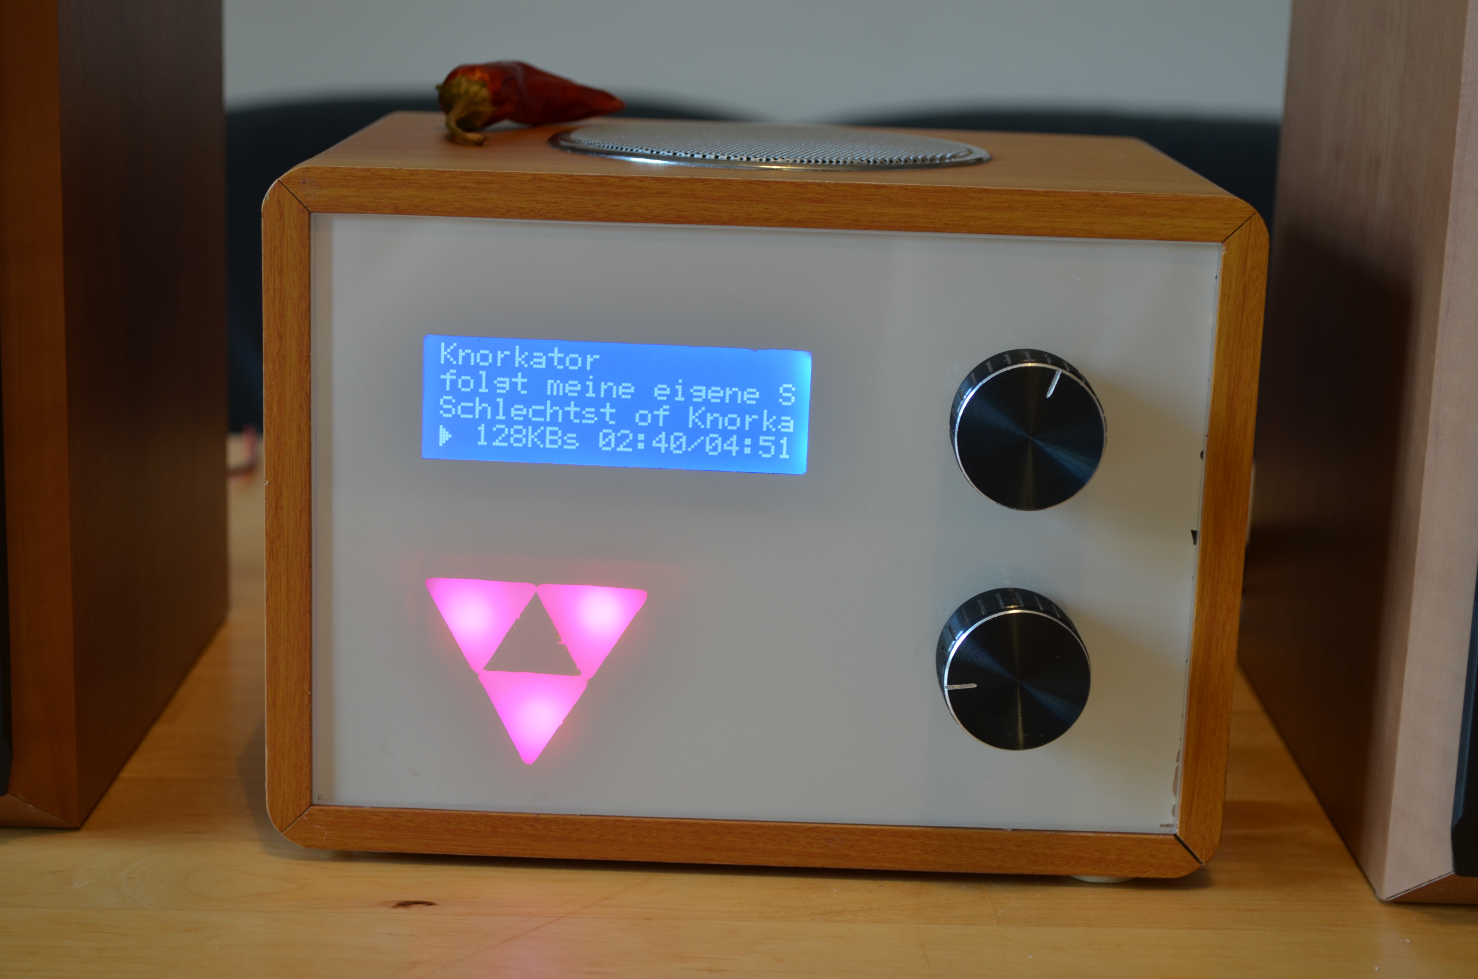
\includegraphics[width=0.5\textwidth]{images/front_3.png}
  \caption{Aktueller Prototyp}
  \label{fertig}
\end{figure}

\newpage 

Abbildung \ref{fertig} zeigt den \emph{Eulenfunk} Prototypen, welcher im
Zeitraum von drei Wochen im Rahmen des Hardwaresysteme Kür--Projekts
entstanden ist. Auf Vimeo\footnote{Eulenfunk Prototyp:
  \url{https://vimeo.com/171646691}} ist ein Video des aktuellen
Prototypen zu sehen.

\section{Verwendete Software}\label{verwendete-software}

Für die Entwicklung und Dokumentation wurden folgende \emph{GNU/Linux}
Tools verwendet:

\begin{itemize}
\tightlist
\item
  \emph{Pandoc/LaTeX} (Dokumentation)
\item
  \emph{Vim} (Softwareentwicklung)
\item
  \emph{Fritzing} (Schaltpläne).
\end{itemize}

\chapter{Motivation}\label{motivation}

\section{Private Situation}\label{private-situation}

Die Autoren dieses Projekts leben in einer Wohngemeinschaft zusammen.
Die Küche ist der Ort an welchem gemeinsam gekocht und gespeist wird.
Für eine angenehme Atmosphäre und als Nachrichten--Quelle sorgte in der
Küche früher ein Analog--Radio der Firma \emph{AEG}, welches aufgrund
der schlechten Empfangsqualität durch eine Kombination aus »alter
Stereoanlage«, »altem Raspberry Pi« und einem »alten Thinkpad x61t«
ersetzt wurde. In dieser Kombination fungierte die Stereoanlage als
Soundausgabe--Komponente, auf dem \emph{Raspberry Pi} lief der
Linux--basierte Player Volumio\footnote{Volumio:
  \url{https://volumio.org/}}, welcher mit dem Touchscreen des
\emph{Thinkpad x61t} über eine Weboberfläche gesteuert wurde. Diese
Kombination hat zwar funktioniert, jedoch war sie alles andere als
benutzerfreundlich, da zuerst die Stereoanlage und der Laptop
eingeschaltet werden mussten und eine WLAN--Verbindung zum
\emph{Raspberry Pi}--Player hergestellt werden musste. Diese Situation
weckte den Wunsch nach einer komfortableren Lösung, beispielsweise ein
Internetradio auf Basis des \emph{Raspberry Pi}.

\section{Kommerzielle Produkte}\label{kommerzielle-produkte}

Kommerzielle Anbieter von Internetradios gibt es wie Sand am Meer. Die
Preisspanne liegt hier zwischen \EUR{30} und mehreren hundert Euro. Der
Funktionsumfang sowie die Wiedergabequalität ist hier von Hersteller zu
Hersteller und zwischen den verschiedenen Preisklassen sehr
unterschiedlich. Einen aktuellen Überblick aus dem Jahr 2016 über
getestete Modelle gibt es beispielsweise online unter
\emph{bestendrei.de}\footnote{Test von Internetradios:
  \url{http://www.bestendrei.de/elektronik/internetradio/}}.

Das \emph{Problem} bei den kommerziellen Anbietern ist, dass man hier
jeweils an die vorgegebenen Funktionalitäten des Herstellers gebunden
ist. Bei einem Do--It--Yourself--Projekt auf Basis Freier Software
beziehungsweise eines freien Hardwaredesigns, hat man die Möglichkeit
alle gewünschten Funktionalitäten --- auch Features die von keinem
kommerziellen Anbieter unterstützt werden --- zu integrieren. Beispiele
für Funktionalitäten, welche bei kommerziellen Produkten nur schwer
beziehungsweise vereinzelt zu finden sind:

\begin{itemize}
\tightlist
\item
  Unterstützung bestimmter WLAN--Authentifizierungsstandards
\item
  Einhängen von benutzerdefinierten Dateifreigaben wie \emph{Samba},
  \emph{NFS}, \emph{SSHFS}
\item
  Unterstützung verschiedener \emph{lossy} und \emph{lossless} Formate
  \emph{OGG VORBIS}, \emph{FLAC}, u.a.
\item
  Integration verschiedener Dienste wie beispielsweise \emph{Spotify}
\item
  Benutzerdefinierte Anzeigemöglichkeiten (Uhrzeit, Wetter, et. cetera.)
\end{itemize}

\chapter{Projektspezifikation}\label{projektspezifikation}

\section{Hardwareanforderungen}\label{hardwareanforderungen}

Das Radio soll dem Benutzer folgende Hardwarekonfigurationsmöglichkeiten
bieten:

\begin{itemize}
\tightlist
\item
  Anschluss passive Lautsprecher/Kopfhörer möglich
\item
  Lautstärkeregelung über Hardware möglich
\item
  Verwendung des internen Lautsprechers des alten Radios
\item
  Statusinformationen zum aktuellen Lied beispielsweise über ein LCD
\item
  LEDs als Statusanzeige und/oder als Visualisierungsvariante von
  Musik\footnote{Moodbar: \url{https://en.wikipedia.org/wiki/Moodbar}}
\item
  USB--Anschlussmöglichkeit für externe Datenträger
\end{itemize}

\section{Softwareanforderungen}\label{softwareanforderungen}

Die Software soll generisch gehalten werden um eine möglichst einfache
Erweiterbarkeit zu gewährleisten.

TODO Eule: Hier was zu Menü--Steuerung schrieben und Umfang?

\section{Optik-- und
Usability--Anforderungen}\label{optik-und-usabilityanforderungen}

Die Eingabe--Peripherie soll möglichst einfach gehalten werden, um eine
\emph{schöne} Produkt--Optik zu gewährleisten, dabei sollen folgende
Anforderungen erfüllt werden:

\begin{itemize}
\tightlist
\item
  Minimale sowie ansprechende Bedienelemente
\item
  Funktionales, zweckgebundenes \emph{Design}
\item
  \emph{Retro--Look}-Aussehen wünschenswert
\end{itemize}

Das \emph{Design} soll im Grunde \emph{minimalistisch} gehalten werden,
das heißt, es sollen aufgrund der Übersichtlichkeit nur so wenige
»Bedienelemente« wie nötig angebracht werden.

\chapter{Hardware}\label{hardware}

\section{Komponenten und Bauteile}\label{komponenten-und-bauteile}

Folgende Hardwarekomponenten oder Bauteile sind bereits vorhanden oder
müssen noch erworben werden:

\textbf{Vorhanden:}

\begin{itemize}
\tightlist
\item
  Altes Gehäuse AEG 4104 Küchenradio\footnote{AEG Küchenradio 4104:
    \url{https://www.amazon.de/AEG-MR-4104-Desgin-Uhrenradio-buche/dp/B000HD19W8}}
\item
  \emph{Raspberry Pi} aus dem Jahr 2012
\item
  LCD--Anzeige (Altbestände u. Arduino--Kit)
\item
  Kleinbauteile wie LEDs, Widerstände
\item
  USB--Hub für Anschluss von beispielsweise ext. Festplatte
\item
  USB--Soundkarte
\item
  Wi--Fi--Adapter
\item
  Netzteil (diverse 5V, 2mA)
\end{itemize}

\textbf{Muss noch erworben werden:}

\begin{itemize}
\tightlist
\item
  Audioverstärker
\item
  Drehimpulsregler
\item
  Kunststoffabdeckung für Front
\item
  Farbe (Lack)
\item
  Drehknöpfe für das Gehäuse
\end{itemize}

TODO Katze: Beschreibung an Diagrammpfeile

\begin{figure}[h!]
  \centering
  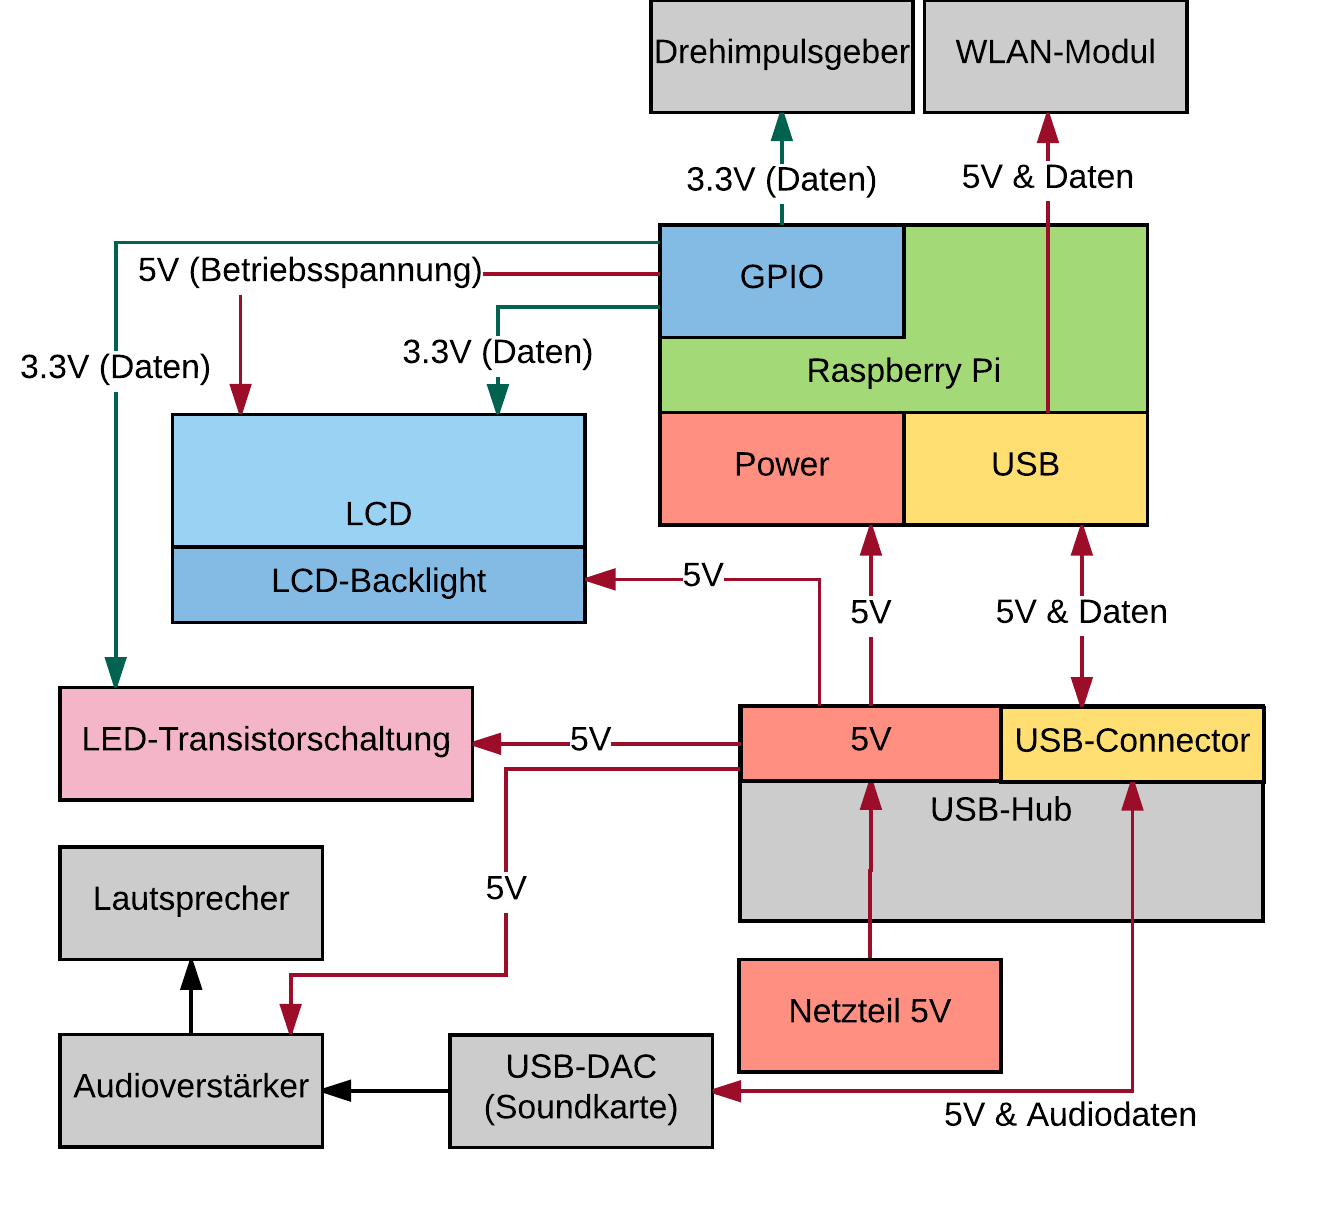
\includegraphics[width=0.7\textwidth]{images/uebersicht.png}
  \caption{Grobe Übersicht der verwendeten Komponenten im Zusammenspiel}
  \label{uebersicht}
\end{figure}

Abbildung \ref{uebersicht} zeigt eine konzeptuelle Übersichts des
Zusammenspiels der einzelnen Komponenten.

\section{Raspberry Pi}\label{raspberry-pi}

Der vorhandene \emph{Raspberry Pi} ist aus dem Jahr 2012. Die genaue
Hardware--Revision kann auf Linux unter \texttt{proc} ausgelesen werden,
siehe auch {[}1{]}, Seite 46:

\begin{Shaded}
\begin{Highlighting}[]

    \NormalTok{$ }\KeywordTok{cat} \NormalTok{/proc/cpuinfo }
    \KeywordTok{processor}       \NormalTok{: 0}
    \KeywordTok{model} \NormalTok{name      : ARMv6-compatible processor rev 7 (v6l)}
    \KeywordTok{BogoMIPS}        \NormalTok{: 697.95}
    \KeywordTok{Features}        \NormalTok{: half thumb fastmult vfp edsp java tls }
    \KeywordTok{CPU} \NormalTok{implementer : 0x41}
    \KeywordTok{CPU} \NormalTok{architecture: 7}
    \KeywordTok{CPU} \NormalTok{variant     : 0x0}
    \KeywordTok{CPU} \NormalTok{part        : 0xb76}
    \KeywordTok{CPU} \NormalTok{revision    : 7}

    \KeywordTok{Hardware}        \NormalTok{: BCM2708}
    \KeywordTok{Revision}        \NormalTok{: 0003}
    \KeywordTok{Serial}          \NormalTok{: 00000000b8b9a4c2}
\end{Highlighting}
\end{Shaded}

Laut Tabelle unter {[}1{]}, Seite 45 handelt es sich hierbei um das
Modell B Revision 1+ mit 256MB RAM.

Je nach Raspberry Revision sind die Pins teilweise unterschiedlich
belegt. Seit Modell B, Revision 2.0 ist noch zusätzlich der P5 Header
dazu gekommen. Abbildung \ref{gpio}\footnote{Bildquelle:
  \url{http://www.raspberrypi-spy.co.uk/2012/06/simple-guide-to-the-rpi-gpio-header-and-pins/\#prettyPhoto}}
zeigt die GPIO--Header des \emph{Raspberry Pi} Modell B Revision 1+.

\subsection{GPIO--Schnittstelle}\label{gpioschnittstelle}

\begin{figure}[h!]
  \centering
  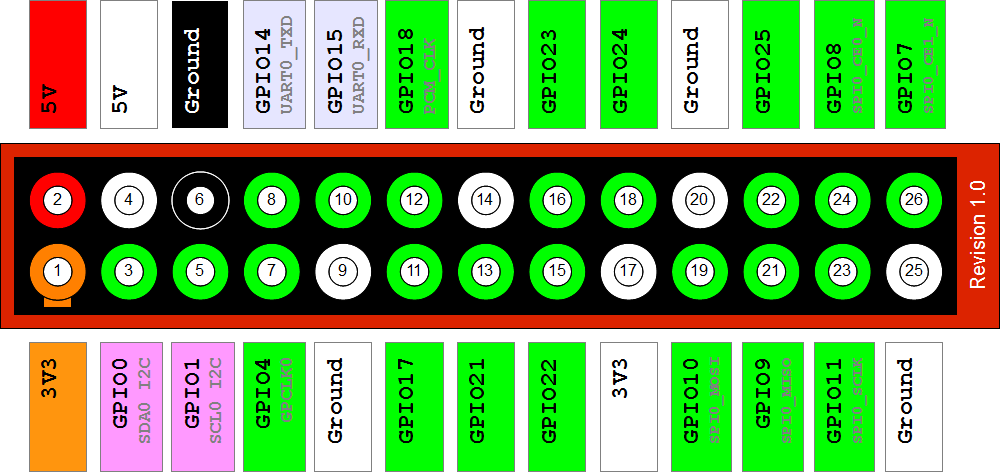
\includegraphics[width=0.7\textwidth]{images/gpio.png}
  \caption{GPIO-Header des Raspberry Pi Modell B Rev 1.0+}
  \label{gpio}
\end{figure}

\subsubsection{GPIO--Pinbelegung und
Funktionalität}\label{gpiopinbelegung-und-funktionalituxe4t}

Die GPIO--Pins des \emph{Raspberry Pi} haben eine Logikspannung von 3.3V
und sind pro GPIO--Pin mit max. 16mA belastbar. Der der gesamte
GPIO--Header sollte mit nicht mehr als 50mA belastet werden, da es
darüber hinaus zu Hardwareschäden kommen kann (vgl. {[}1{]}, Seite 20
ff.).

Die \emph{Logik--Pegel} der GPIO--Pins sind beim \emph{Raspberry Pi} wie
folgt definiert {[}1{]}, Seite 23 ff.:

\begin{itemize}
\item
  \textless{}= 0,8V, input low
\item
  \begin{quote}
  = 1,3V, input high
  \end{quote}
\end{itemize}

Die Ansteuerung Ansteuerung von LED über GPIO erfolgt binär. Das heißt,
dass die LED entweder aus (GPIO low) oder an sein kann (GPIO high).

TODO: ELCH? In der »analogen« Welt ist es jedoch möglich eine LED über
das Senken der Spannung zu dimmen. Um ein Dimmen in der digitalen Welt
zu erreichen wird ein Modulationsverfahren angewandt, welches
Pulsweitenmodulation heißt. Hierbei wird\ldots{}TODO: ELCH? Unter
{[}2{]}, Seite 121 ff. und {[}3{]}, Seite 421 ff. finden sich weitere
Integration.

Software PWM unter {[}4{]}, Seite 183 ff. zeigt beispielsweise eine 6\%
CPU--Last pro GPIO--Pin bei einer PWM--Softwareimplementierung. TODO:
ELCH?

\section{LCD--Anzeige}\label{lcdanzeige}

Um dem Benutzer Informationen beispielsweise über das aktuell gespielte
Lied anzeigen zu können, soll eine LCD--Anzeige verbaut werden. In den
privaten Altbeständen finden sich folgende drei Hitachi
hd44780--kompatible Modelle:

\begin{itemize}
\tightlist
\item
  Blaues Display, 4x20 Zeichen, Bolymin BC2004A
\item
  Blaues Display, 2x16 Zeichen, Bolymin BC1602A
\item
  Grünes Display, 4x20 Zeichen, Dispalytech 204B
\end{itemize}

Für \emph{Eulenfunk} wurde das blaue 4x20 Display --- aufgrund der
größeren Anzeigefläche und Farbe --- gewählt.

\subsection{Anschlussmöglichkeiten}\label{anschlussmuxf6glichkeiten}

Ein LCD Display kann an den Raspberry PI über auf verschiedene Art und
Weise angeschlossen werden. Anschlussmöglichkeiten für eine LCD--Anzeige
wären beispielsweise:

\begin{itemize}
\tightlist
\item
  GPIO direkt (parallel)
\item
  I2C--Bus (seriell)
\item
  SPI--Bus (seriell)
\end{itemize}

Die serielle Anschlussmöglichkeit bietet den Vorteil dass weniger
Datenleitungen (GPIO--Pins) verwendet werden. Für den parallelen Betrieb
des Displays werden mindestens sechs GPIO--Pins benötigt, für den
seriellen Anschluss über I2C lediglich nur zwei.

Da für den seriellen Betrieb beispielsweise über den I2C--Bus
zusätzliche Hardware benötigt wird, wird die parallele Ansteuerung über
die GPIO--Pins bevorzugt. Weitere Informationen zum seriellen Betrieb
über I2C sind unter {[}5{]}, Seite 61, ff. zu finden.

\begin{figure}[h!]
  \centering
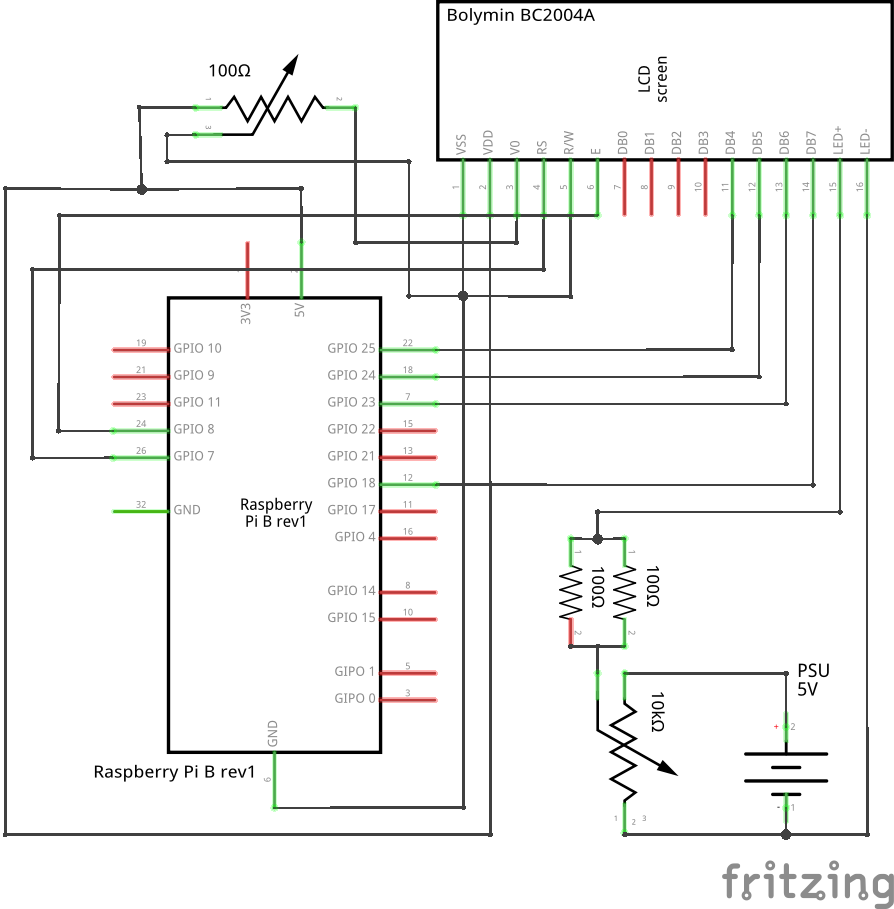
\includegraphics[width=0.7\textwidth]{images/lcdraspi.png}
  \caption{Verdrahtung von LCD und Raspberry Pi.}
  \label{lcd}
\end{figure}

Das Display arbeitet mit einer Logik--Spannung von 3.3V - 5V. Da die
GPIO--Pins jedoch eine High--Logik von 3,3V aufweisen, würde man hier in
der Regel einen Pegelwandler bei bidirektionaler Kommunikation und 5V
benötigen. Da wir aber nur auf das Display zugreifen und die GPIO--Pins
nicht schreibend zugegriffen wird kann ein Betrieb des Displays auch mit
5V erfolgen. Beim 3.3V Betrieb welcher laut Datenblatt auch möglich sein
soll, hat das Display leider nur eine sehr schwachen beziehungsweise
unzureichenden Darstellungskontrast gehabt, weswegen der 5V Betrieb
gewählt wurde.

Die Hintergrundbeleuchtung des Displays wurde direkt über ein
Potentiometer mit 10K\(\Omega\) an die 5V Spannungsversorgung
angeschlossen. Es wurde hier direkt die Speisung vom Netzteil gewählt um
den GPIO--Header nicht unnötig zu belasten.

Laut Datenblatt\footnote{Datenblatt Bolymin BC2004A:
  \url{http://www.dema.net/pdf/bolymin/BC2004A-series_VER04.pdf}} kann
die Hintergrundbeleuchtung entweder mit 3.4V ohne Vorwiderstand oder mit
5V bei einem 27\(\Omega\) Widerstand betrieben werden. Damit das Display
beim herunter geregeltem Potentiometer keinen Schaden nimmt, wurden
zusätzlich zwei Widerstände mit 100\(\Omega\) (parallel geschaltet =
50\(\Omega\)) zwischen Display und Potentiometer gehängt.

Das der resultierende Gesamtwiderstand ohne Potentiometer beträgt in
diesem Fall \(\approx\) 50 \(\Omega\):

\[  R_{ges} = \frac{R_1 \times R_2}{R_1 + R_2} = \frac{100\Omega \times 100\Omega}{100\Omega + 100\Omega} = 50\Omega \]

\section{Rotary--Switch}\label{rotaryswitch}

Für eine minimale Anzahl an Bedienelementen zu erhalten, wird bei
\emph{Eulenfunk} ein Drehimpulsgeber mit Schalter gewählt. Für erste
Testzwecke wurde vom Herrn Schäferling ein \emph{ALPS STEC12E08}
bereitgestellt. Dieser wurde im Laufe der Entwicklung durch einen
\emph{ALPS STEC11B09}\footnote{Drehimpulsgeber ALPS STEC11B09:
  \url{https://www.reichelt.de/Drehimpulsgeber/STEC11B09/3/index.html?ACTION=3&GROUPID=3714&ARTICLE=73915}}
ersetzt, da dieser mittels Mutter und Schraube am Gehäuse besser
befestigt werden kann.

Der verwendete Drehimpulsgeber hat insgesamt fünf Anschlüsse. Zwei
Signalleitungen (A und B), zwei mal \emph{GND} (für Drehgeber und
Schalter jeweils eine) und einen Anschluss für den Schalter. Beim drehen
eines Drehimpulsgebers wird ein Rechtecksignal generiert. Je nach Muster
der beiden Datensignale A oder B, kann entschieden werden ob es sich um
eine Rechts-- oder Linksdrehung handelt. Siehe {[}6{]}, Seite 361 ff.
für weitere Hintergrundinformationen zu Drehimpulsgeber.

Abbildung \ref{alps} zeigt den Anschluss des Drehimpulsgebers am
\emph{Raspberry Pi}.

\begin{figure}[h!]
  \centering
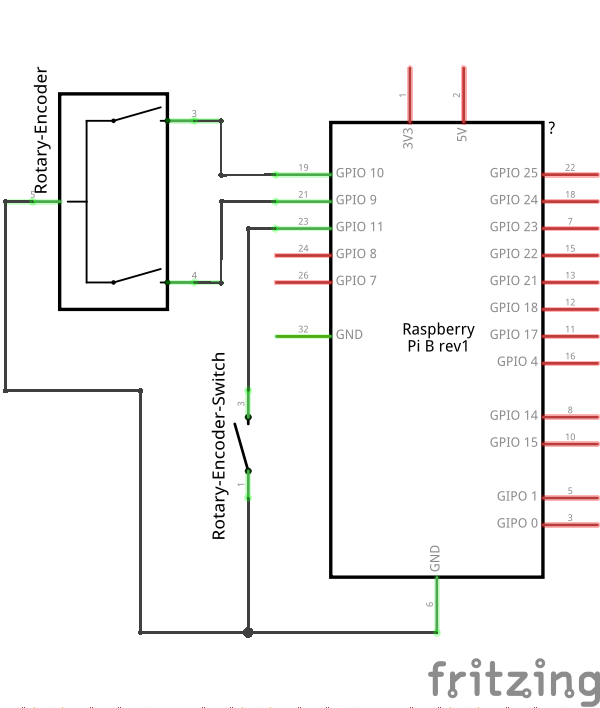
\includegraphics[width=0.6\textwidth]{images/rotary.png}
  \caption{Drehimpulsgeber--Anschluss an den Raspberry Pi, Abbildung zeigt
  Kombination aus Potentiometer und Schalter.}
  \label{alps}
\end{figure}

\section{Soundkarte}\label{soundkarte}

Die interne Soundkarte des \emph{Raspberry Pi} ist über eine triviale
Pulsweitenmodulation realisiert. Die einfache Schaltung soll hier laut
Internetquellen\footnote{Raspberry Pi onboard Sound:
  \url{http://www.crazy-audio.com/2013/11/quality-of-the-raspberry-pi-onboard-sound/}}eine
sehr niedrige Audioqualität bieten.

Aus diesem Grund wird bei \emph{Eulenfunk} auf das USB--Audio--Interface
\emph{BEHRINGER U-PHONO UFO202}\footnote{BEHRINGER U-PHONO UFO202 Audio
  Interface:
  \url{http://www.produktinfo.conrad.com/datenblaetter/1300000-1399999/001370864-an-01-de-BEHRINGER_UFO_202_AUDIOINTERFACE.pdf}}
gesetzt.

\section{Audioverstärkermodul}\label{audioverstuxe4rkermodul}

Da eine Soundkarte in der Regel zu wenig Leistung hat um einem
Lautsprecher »vernünftig« anzusteuern wird ein Audioverstärker benötigt.
Da neben dem Anschluss von externen Lautsprechern auch eine
Lautstärkeregelung über ein Poti erfolgen soll, ist die Entscheidung
einfachheitshalber auf ein Audioverstärker--Modul auf Basis vom
PAM8403\footnote{Verstärkermodul:
  \url{https://www.amazon.de/5V-Audioverstärker-Digitalendstufenmodul-Zweikanalige-Stereo-Verstärker-Potentiometer/dp/B01ELT81A6}}
Stereo-Verstärker mit Potentiometer gefallen. Eine
Do--It--Yourself--Alternative wäre ein Transistor--basierter
Audio--Verstärker, hier gibt es online diverse Bauanleitungen\footnote{Transistor--Verstärker:
  \url{http://www.newsdownload.co.uk/pages/RPiTransistorAudioAmp.html}}.

Das Audioverstärker--Module hat folgende Anschlusspins:

\begin{itemize}
\tightlist
\item
  Left--In, Right--In, GND
\item
  5V+ und GND (Betriebsspannung)
\item
  Left--Side--Out (+), Left--Side--Out (-)
\item
  Right--Side--Out (+), Right--Side--Out (-)
\end{itemize}

Laut diverser Onlinequellen\footnote{PAM8403 Mono--Betrieb:
  http://electronics.stackexchange.com/questions/95743/can-you-bridge-or-parallel-the-outputs-of-the-pam8403-amplifier},
dürfen die Ausgänge für einen Mono--Betrieb eines auf dem
PAM8403--basierten Verstärkers nicht parallel geschaltet werden. Aus
diesem Grund kommt ein ein 4--poliger
\emph{EIN--EIN--Kippschalter}\footnote{Kippschalter 4--polig EIN--EIN:
  \url{http://www.reichelt.de/Kippschalter/MS-500P/3/index.html?&ACTION=3&LA=2&ARTICLE=13172&GROUPID=3275&artnr=MS+500P}}
zum Einsatz. So kann zwischen dem internen Lautsprecher (Mono--Betrieb)
und den externen Stereo Lautsprecher--Anschlüssen sauber per Hardware
hin und her geschaltet werden.

Damit im Mono--Betrieb nicht nur ein Kanal verwendet wird, ermöglicht
\emph{Eulenfunk} das umschalten zwischen Mono-- und Stereo--Betrieb in
Software.

\section{LED--Transistorschaltung}\label{ledtransistorschaltung}

Die Ansteuerung einer LED mittels GPIO--Pin ist recht simpel. Sollen
jedoch mehrere LEDs angesteuert werden, so wird in der Regel pro LED ein
GPIO--Pin benötigt. LEDs sollten nie ohne Vorwiderstand an den
\emph{Raspberry Pi} angeschlossen werden, da durch den hohen Stromfluss
die LED beschädigt werden könnte. Weiterhin muss bei LEDs auch auf die
Polung geachtet werden, die abgeflachte Seite --- meist mit dem kürzerem
Beinchen -- ist in der Regel die Kathode (Minuspol). Abbildung \ref{led}
zeigt exemplarisch den Anschluss einer \emph{classic LED rot}\footnote{Datenblatt
  mit verschiedenen LED--Typen:
  \url{https://www.led-tech.de/de/5mm-LEDs_DB-4.pdf}}, mit einer
Flussspannung von \(U_{LED}\) \(\approx\) 2V, die mit einem Strom von
\(I_{LED}\) = 20 mA gespeist werden soll. Die Berechnung des
Vorwiderstandes erfolgt nach folgender Formel:

\[R_{LED} = \frac{U_{GPIO}-U_{LED}}{I_{LED}} = \frac{3.3V - 2V}{20mA}   \approx 65\Omega\]

\textbf{Hinweis:} Da ein GPIO--Pin aber mit nur max. 16mA belastet
werden sollten, sollte in unserem Beispiel durch 16mA anstatt 20mA
geteilt werden um den max. Stromfluss auf 16mA zu begrenzen. In diesem
Fall würden wir auf \(\approx\) 82\(\Omega\) kommen.

Da Widerstände meistens in fest vorgegebenen Größen vorhanden sind, kann
im Fall eines nicht exakt existierenden Widerstandswertes einfach der
nächsthöhere Widerstandswert genommen werden. Im Beispiel wird ein
\(100\Omega\) Widerstand verwendet.

Weitere Beispiele und Grundlagen zur Reihen-- und Parallelschaltung von
LEDs können online beispielsweise unter \emph{led-treiber.de}\footnote{Beispiele
  zur Ansteuerung von LEDs:
  \url{http://www.led-treiber.de/html/vorwiderstand.html}} eingesehen
werden.

\begin{figure}[h!]
  \centering
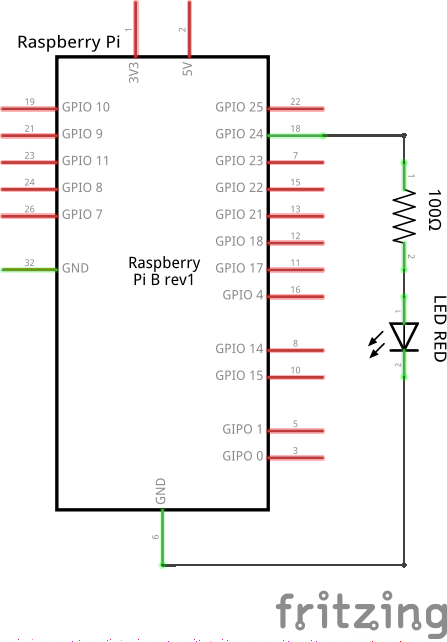
\includegraphics[width=0.5\textwidth]{images/led.png}
  \caption{Anschluss eine roten LED mit Vorwiderstand am Raspberry Pi GPIO--Pin}
  \label{led}
\end{figure}

Je nach Typ und Farbe ist der benötigte Strom um ein vielfaches höher
wie in unserem Beispiel. Die in \ref{led} abgebildete LED kann vom
GPIO--Pin nur einen max. Strom von 16 mA beziehen

In \emph{Eulenfunk} sollen mehrere intensiv leuchtende LEDs verbaut
werden. Da die GPIO--Pins in ihrer Leistung sehr begrenzt ist, würde es
sich anbieten eine externe Stromquelle zu verwenden. Um die Speisung
über eine externe Stromquelle zu ermöglichen kann eine
Transistorschaltung verwendet werden (vgl. {[}7{]}, Seite 217 ff.).

Für die Transistorschaltung wurden vom Herrn Schäferling NPN (BC547C)
und PNP (BC557C) bereitgestellt. Für den ersten Testaufbau wurde der
PNP--Transistor und eine RGB--LED\footnote{RGB-LED Common Cathode:
  \url{http://download.impolux.de/datasheet/LEDs/LED 0870 RGB 5mm klar 10000mcd.pdf}}
mit gemeinsamen Minuspol verwendet. Beim Test--Aufbau mit einem
PNP--Transistor ist aufgefallen, dass die LED ständig geleuchtet hat.
Eine kurze Recherche hat ergeben, dass der Transistor permanent
durchgeschaltet war, weil die Spannung an der Basis (GPIO--Pin, 3,3V)
geringer war die die Betriebsspannung für die LED (5V).

Der zweite Anlauf mit dem NPN--Transistor BC547C und einer
RGB--LED\footnote{RGB-LED Common Anode:
  \url{http://download.impolux.de/datasheet/LEDs/LED 09258 RGB 5mm klar 10000mcd_GP.pdf}}
mit gemeinsamen Pluspol hat das gewünschte Ergebnis geliefert.

Da der Hersteller für die von der Hochschule bereitgestellten
Transistoren unbekannt ist, wurden typische Durchschnittswerte für die
Dimensionierung der Restlichen Bauteile verwendet.

Wie es aussieht sind die meisten BC547C Transistor Typen für einen max.
Strom \(I_{CE}\)=100 mA konstruiert. Für die Berechnung des
Basis--Vorwiderstandes ist der Stromverstärkungsfaktor
\(h_{FE}\)\footnote{Stromverstärkungsfaktor:
  \url{http://www.learningaboutelectronics.com/Articles/What-is-hfe-of-a-transistor}}
benötigt. Je nach Hersteller variieren die Werten zwischen 200\footnote{SEMTECH:
  \url{http://pdf1.alldatasheet.com/datasheet-pdf/view/42386/SEMTECH/BC547.html}}
und 400\footnote{Farichild Semiconductor:
  \url{https://www.fairchildsemi.com/datasheets/BC/BC547.pdf}}. Da der
maximale Laststrom \(I_{CE}\) pro Transistor beträgt 80 mA (3 LEDs je
max. 20mA), sieht die Berechnung des Basisstroms wie folgt aus:

\[I_{Basis} = \frac{I_{CE}}{h_{FE}} = \frac{0.08A}{300} \approx 270\mu A\]

Der BC547C Transistor benötigt eine durchschnittliche \(U_{BE}\) = 0,7V
zum durchschalten. Die GPIO-Pins des \emph{Raspberry Pi} haben einen
Spannungspegel von 3.3V. Daraus ergibt sich folgende Berechnung des
Basis--Vorwiderstandes:

\[R_{Basis} = \frac{U_{GPIO} - U_{Basis}}{I_{Basis}} = \frac{3,3V - 0,7V}{270\mu A} = 9629 \Omega \approx 10k \Omega \]

\begin{figure}[h!]
  \centering
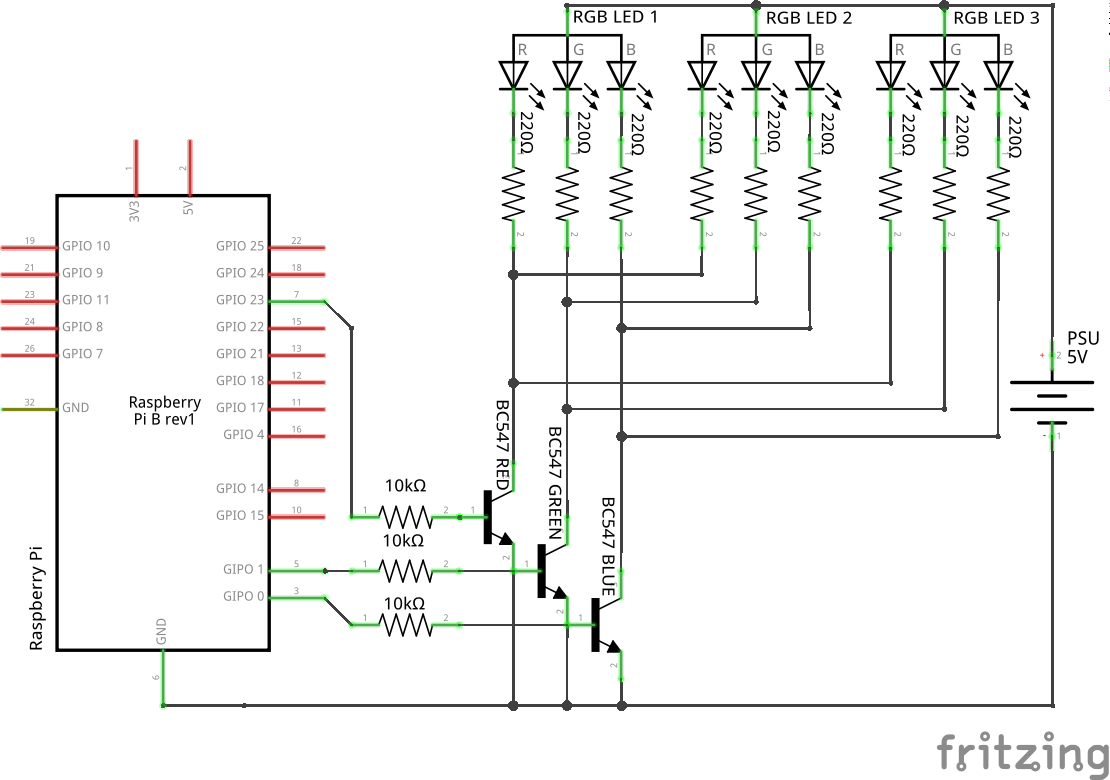
\includegraphics[width=0.9\textwidth]{images/transistorled.png}
  \caption{Transistor--RGB--LED Schaltung}
  \label{transled}
\end{figure}

Die in Abbildung \ref{transled} gelisteten LED--Vorwiderstände ergeben
sich aufgrund der verschiedenen Spannungen der unterschiedlichen
Farben\footnote{RGB-LED Common Anode:
  \url{http://download.impolux.de/datasheet/LEDs/LED 09258 RGB 5mm klar 10000mcd_GP.pdf}}.
Die Berechnung für den Vorwiderstand pro LED schaut am Beispiel der
Farbe blau (\(U_{LED} = 3,15V, I_{LED} = 20mA\)) wie folgt aus:

\[R_{LED} = \frac{U_{Betriebsspannung} - U_{LED}}{I_{LED}} = \frac{5V - 3,15V}{20mA} =92.5 \approx 100\Omega\]

\section{USB--Hub und Netzteil}\label{usbhub-und-netzteil}

Der \emph{Raspberry Pi} hat in unserer Revision nur zwei
USB--Schnittstellen, diese sind bereits durch die Hardware--Komponenten
USB--DAC (Soundkarte) und das Wi--Fi--Modul belegt. Um den Anschluss
eines externen Datenträgers, auch mit größerer Last wie beispielsweise
einer Festplatte zu ermöglichen wird ein aktiver USB--Hub benötigt.

Für diesen Einsatzzweck wird aus den Altbeständen ein \emph{LogiLink 4
Port USB 2.0 HUB} verwendet. Viele billig-Hubs arbeiten hier entgegen
der USB--Spezifikation und speisen zusätzlich über die
USB--Schnittstellen den \emph{Raspberry Pi}. Dieses Verhalten wurde
bemerkt, also der \emph{Raspberry Pi} ohne Power--Connector alleine mit
nur der USB--Verbindung zum Hub bootete.

Bei der Speisung über die USB--Schnittstelle wird die interne
Sicherungsschaltung des \emph{Pi} umgangen, deswegen wird in der Regel
von einem Betrieb eines USB--Hub mit \emph{backfeed} abgeraten (vgl .
{[}8{]}, Seite 26 ff.). Für den Prototypen wird jedoch der USB--Hub und
das dazugehörige Netzteil für den Betrieb von \emph{Eulenfunk}
verwendet. Das Netzteil ist für 5V bei max. 2A ausgelegt.

\textbf{Nachtrag:} Die Speisung über das 5V, 2A des USB--Hubs ist recht
instabil. Bei Lastspitzen kommt es anscheinend zu Störeinwirkungen die
sich auf die GPIO--Peripherie auswirken (LCD--Anzeige rendert inkorekt).
Ein weiterer Punkt sind Störfrequenzen, welche teilweise in Form von
Störgeräuschen die Audioausgabe überlagern (Hintergrundgeräusche beim
Einschalten aller LEDs). Insgesamt wurden drei Netzteile --- jeweils 5V,
2A ---ausprobiert. Von diesen war lediglich ein einziges als
\enquote{akzeptabel} einzustufen. Die restlichen zwei führen bei
Lastspitzen zu Problemen (Abstürze, fehlerhaftes Rendering auf Display,
GPIO--Flips, et cetera). Das \emph{backfeed} des USB--Hubs scheint die
genannten Probleme teilweise zu verstärken (vgl . {[}8{]}, Seite 27).

\section{Gehäuse}\label{gehuxe4use}

\subsection{Vorderseite}\label{vorderseite}

Abbildung \ref{ral} zeigt ein Muster der Gehäusefront--Farbe
hellelfenbeinweiß RAL 1015. Dieser Farbton wird für die Front verwendet
um \emph{Eulenfunk} einen dezenten »Retro«--Look verpassen.

\begin{figure}[h!]
  \centering
  
\includegraphics[width=0.3\textwidth]{images/ral_soft.png}
  \caption{Muster RAL1015, hellelfenbeinweiß}
  \label{ral}
\end{figure}

Das Plexiglas für die Front wurde von der Firma \emph{ira-Kunststoffe}
in Schwarzenbach/Saale zugeschnitten. In der Plexiglasfront wurden mit
Hilfe vom Herrn Schäferling zwei 5mm Löcher (Drehimpulsgeber,
Lautstärkeregler--Poti) gebohrt. Anschließend wurde die Plexiglas--Front
von der Innenseite lackiert\footnote{Buntlack, hellelfenbein:
  \url{http://www.obi.de/decom/product/OBI_Buntlack_Spray_Hellelfenbein_hochglaenzend_150_ml/3468725}},
hierbei wurden die Flächen für LCD und die drei LEDs abgelebt. Zudem
werden schwarze Knöpfe in Alu--Optik mit \(\diameter\) 30mm für den
Lautstärkeregler und den Drehimpulsgeber verwendet.

\subsection{Hinterseite}\label{hinterseite}

Für die Hinterseite wird die alte Abdeckung verwendet. Diese musste
Teilweise leicht modifiziert werden. An dieser befinden sich zwei Potis
für Kontrastregelung und Hintergrundbeleuchtung des LCD, eine
USB--Female--Kabelpeitsche, zwei Cinch Stecker für externe Lautsprecher
und ein Kippschalter zum Umschalten zwischen internen und externen
Lautsprechern.

\section{Betriebssystem}\label{betriebssystem}

Mittlerweile gibt es für den \emph{Raspberry Pi} viele offiziell
zugeschnittene Betriebssysteme (vgl. {[}9{]}, Seite 29 ff., {[}10{]},
Seite 47 ff.). Bei den den Linux Distributionen ist \emph{Raspbian} eine
der bekanntesten Distribution -- welche auf \emph{Debian} basiert.
\emph{Raspbian} bringt ein komplettes Linux--basiertes System mit
grafischer Benutzeroberfläche mit sich.

Neben den unter {[}9{]}, Seite 29 ff. genannten Distributionen gibt es
mittlerweile auch Windows 10 IoT (Internet of Things) für den
\emph{Raspberry Pi}. Dieses speziell für den Embedded Bereich
ausgerichtete Windows benötigt jedoch eine ARMv7--CPU als
Mindestanforderung, was unseren »alten Raspberry« ausschließen würde.
Außerdem wäre für uns eine proprietäre Lösung ein K.O.--Kriterium, da
diese alle Vorteile von Freier Software zunichte machen würde.

\subsection{Wahl des Betriebssystem}\label{wahl-des-betriebssystem}

\emph{Arch Linux ARM}\footnote{Arch Linux ARM:
  \url{https://archlinuxarm.org/}} ist eine minimalistische und sehr
performante Linux--Distribution welche im Gegensatz zu \emph{Raspbian}
ohne Desktop--Umgebung geliefert wird (vgl. {[}11{]}, Seite 13 ff.)
Darüber hinaus ist \emph{Arch Linux} ein bekannter Vertreter von
Rolling--Release--Distributionen. Ein weiterer Vorteil für unseren
Einsatzzweck hier ist bei \emph{Arch Linux} das \emph{AUR} (Arch User
Repository)\footnote{Arch User Repository:
  \url{https://aur.archlinux.org/}}, dieses erlaubt es eigene Software
auf eine schnelle und unkomplizierte Weise der Allgemeinheit zur
Verfügung zu stellen.

\subsection{Einrichtung des
Grundsystems}\label{einrichtung-des-grundsystems}

Nach der Installation\footnote{Arch Linux Installation für Raspberry Pi:
  https://archlinuxarm.org/platforms/armv6/raspberry-pi\#installation}
und dem ersten Booten des Grundsystems muss die Netzwerk--Schnittstelle
konfiguriert werden. Arch Linux ARM bietet mit \emph{netctl} ein
Profil--basierte Konfigurationsmöglichkeit. Ein Profil kann über das
\emph{ncurses}--basierte Tool \texttt{wifi-menu} erstellt werden. In
unserem Fall wurde das Profil \texttt{wlan0-Phobos} erstellt.
Anschließend kann das erstellte Profil mit \emph{netctl} verwendet
werden.

\textbf{Auflistung der bekannten Profile}

\begin{Shaded}
\begin{Highlighting}[]
    \NormalTok{[}\KeywordTok{wald@eulenfunk} \NormalTok{~]$ netctl list}
      \KeywordTok{eth0-static}
      \KeywordTok{wlan0-Phobos}
\end{Highlighting}
\end{Shaded}

\textbf{Aktivierung des gewünschten Profils}

\begin{Shaded}
\begin{Highlighting}[]
    \CommentTok{# Starten des gewünschten Profils}
    \NormalTok{[}\KeywordTok{wald@eulenfunk} \NormalTok{~]$ netctl start wlan0-Phobos}

    \NormalTok{[}\KeywordTok{wald@eulenfunk} \NormalTok{~]$ netctl list}
      \KeywordTok{eth0-static}
    \KeywordTok{*} \NormalTok{wlan0-Phobos}

    \CommentTok{# Profil über System-Reboot hinweg aktivieren }
    \NormalTok{[}\KeywordTok{wald@eulenfunk} \NormalTok{~]$ netctl enable wlan0-Phobos}
\end{Highlighting}
\end{Shaded}

Nun verbindet sich der \emph{Raspberry Pi} nach dem Hochfahren jedes Mal
automatisch mit dem Profil \texttt{wlan0-Phobos}.

\subsection{Abspielsoftware}\label{abspielsoftware}

Für den Betrieb des Internetradios soll der MPD (Music--Player--Daemon)
verwendet werden, da \emph{Eulenfunk} auf einem eigens entwickeltem
MPD--Client basieren soll (mehr zur Eulenkfunk Software siehe Kapitel
Software). Andere Projekte greifen oft auf Abspielsoftware wie den
\emph{MOC} {[}9{]}, Seite 189 ff. oder \emph{mplayer} {[}7{]} Seite 638
ff. zu.

\begin{Shaded}
\begin{Highlighting}[]
    \CommentTok{# Installation des MPD}
    \NormalTok{[}\KeywordTok{root@eulenfunk} \NormalTok{~]$ pacman -Sy mpd mpc ncmpc}
\end{Highlighting}
\end{Shaded}

\chapter{Software}\label{software}

\section{Vorhandene
Softwarelibraries}\label{vorhandene-softwarelibraries}

\section{Überblick der einzelnen
Komponenten}\label{uxfcberblick-der-einzelnen-komponenten}

\section{Softwarearchitektur}\label{softwarearchitektur}

\section{Treiber--Software}\label{treibersoftware}

\subsection{LCD--Treiber}\label{lcdtreiber}

Von Elchen entwickelt.

\subsection{Rotary--Treiber}\label{rotarytreiber}

Von Elchen kopiert.

\subsection{LED--Treiber}\label{ledtreiber}

\begin{itemize}
\tightlist
\item
  Software--PWM
\end{itemize}

\chapter{Zusammenfassung}\label{zusammenfassung}

\section{Ziel erreicht?}\label{ziel-erreicht}

Das selbstgesetzte Ziel --- mit möglichst wenig Aufwand ein
Internetradio auf Basis eines \emph{Raspberry Pi} zu entwickeln --- kann
durchaus als erfolgreich betrachtet werden.

\section{Erweiterungen und alternative
Ansätze}\label{erweiterungen-und-alternative-ansuxe4tze}

\subsection{Allgemein}\label{allgemein}

Der aktuelle Prototyp hat lediglich nur ein Poti um die
Hintergrundbeleuchtung des LCD zu regeln. Ein anderer Ansatz wäre der
Einsatz eines Relais, welches es ermöglichen würde die
LCD--Hintergrundbeleuchtung Software--seitig ein und auszuschalten.

\subsection{Audio--Visualisierung}\label{audiovisualisierung}

Beim Projekt \emph{Eulenfunk} wird die Visualisierung von Musik aufgrund
der begrenzten Zeit und Hardwareressourcen des \emph{Raspberry Pi }über
eine vorberechnete Moodbar--Datei realisiert. Dieser Ansatz funktioniert
bei nicht live gestreamter Musik gut. Bei live gestreamter Musik könnte
für die Visualisierung eine Fast--Fourier--Transformation in Echtzeit
durchgeführt werden. Da jedoch die Ressourcen des \emph{Raspberry Pi}
sehr begrenzt sollte hier auf die Verwendung einer
GPU--beschleunigte--FFT\footnote{GPU--beschleunigte FFT auf dem
  Raspberry Pi: \url{http://www.aholme.co.uk/GPU_FFT/Main.htm}}
zurückgegriffen werden (vgl. {[}12{]}, Seite 657 ff.).

Ein alternativer Ansatz wäre auch die Realisierung einer
Musik--Visualisierung mittels Hardwarekomponenten. Ein möglicher Ansatz
aus Hardware--basierten Hochpass-- und Tiefpassfiltern in Form einer
Disco--Beleuchtung wird unter {[}6{]}, Seite 261 ff. beschrieben.

\subsection{Echtzeit--Uhr}\label{echtzeituhr}

Der \emph{Raspberry Pi} besitzt keine Hardware--Uhr. Aufgrund der
Tatsache dass es sich bei \emph{Eulenfunk} um eine Internet--Radio
handelt wurde auf eine Echtzeituhr (real time clock, RTC) verzichtet, da
sich die Uhr \emph{Eulenfunk} aufgrund der permanenten
Internetverbindung mittels NTP\footnote{Network Time Protocol:
  \url{https://de.wikipedia.org/wiki/Network_Time_Protocol}} über das
Internet synchronisieren kann. Eine Erweiterung um eine Echtzeituhr wird
in {[}5{]}, Seite 145 ff. und {[}4{]}, Seite 77 ff. ausführlich
beschreiben.

\subsection{Fernbedienung}\label{fernbedienung}

Eine weitere Erweiterung wäre die Integration einer Fernbedienung. Diese
ließe sich relativ einfach mittels eine Infrarot--Sensors und
beispielsweise der \emph{lirc}--Bibliothek umsetzen. Siehe auch
{[}10{]}, Seite 190 ff. für weitere Informationen.

\subsection{Batteriebetrieb}\label{batteriebetrieb}

Da die Strom-- beziehungsweise Spannungsversorgung beim \emph{Raspberry
Pi} problematisch ist, wäre auch ein Batterie beziehungsweise
Akkubetrieb möglich. Eine einfache Schaltung für einen Batteriebetrieb
würde sich beispielsweise mit einem \emph{LM7805}--Spannungsregler oder
einem Abwärtswandler realisieren lassen ({[}3{]}, Seite 24 ff.).

\section{Mögliche Verbesserungen?}\label{muxf6gliche-verbesserungen}

\subsection{Alpine Linux}\label{alpine-linux}

Die relativ junge Linux--Distribution \emph{Alpine Linux}\footnote{Alpine
  Linux für Raspberry Pi:
  \url{https://wiki.alpinelinux.org/wiki/Raspberry_Pi}} wäre eine
Mögliche Verbesserung für den Einsatz des Internetradios. Diese
Distribution hat ihren Fokus auf Ressourceneffizienz und
Systemsicherheit. Ein weiterer Vorteil wäre der \texttt{diskless\ mode},
welcher das Komplette Betriebssystem in den Arbeitsspeicher lädt. In
diesem Modus müssen Änderungen mit einem \emph{Alpine Local Backup
(lbu)}--Tool explizit auf die Festplatte geschrieben werden. Das hätte
den Vorteil, dass man die Abnutzung des Flash--Speichers, durch unnötige
Schreib/Lese--Vorgänge, minimieren würde.

\chapter*{Literaturverzeichnis}\label{literaturverzeichnis}
\addcontentsline{toc}{chapter}{Literaturverzeichnis}

\hypertarget{refs}{}
\hypertarget{ref-gay2014raspberry}{}
{[}1{]} W. Gay, \emph{Raspberry Pi Hardware Reference}. Apress, 2014.

\hypertarget{ref-richardson2014make}{}
{[}2{]} M. Richardson and S. Wallace, \emph{Make: Getting Started with
Raspberry Pi}. Maker Media, 2014.

\hypertarget{ref-gay2014mastering}{}
{[}3{]} W. Gay, \emph{Mastering the Raspberry Pi}. Apress, 2014.

\hypertarget{ref-gay2014experimenting}{}
{[}4{]} W. Gay, \emph{Experimenting with Raspberry Pi}. Apress, 2014.

\hypertarget{ref-horan2013practical}{}
{[}5{]} B. Horan, \emph{Practical Raspberry Pi}. Apress, 2013.

\hypertarget{ref-2014projekte}{}
{[}6{]} \emph{Projekte mit dem Raspberry Pi:}. mitp/bhv, 2014.

\hypertarget{ref-exploring}{}
{[}7{]} D. Molloy, in \emph{Exploring Raspberry Pi}, John Wiley \& Sons,
Inc., 2016.

\hypertarget{ref-suehle2014hacks}{}
{[}8{]} R. Suehle and T. Callaway, \emph{Hacks für Raspberry Pi}.
O'Reilly Verlag, 2014.

\hypertarget{ref-pietraszak2014buch}{}
{[}9{]} S. Pietraszak, \emph{Das Buch zu Raspberry Pi mit Linux}.
O'Reilly Verlag, 2014.

\hypertarget{ref-warner2013hacking}{}
{[}10{]} T. Warner, \emph{Hacking Raspberry Pi}. Pearson Education,
2013.

\hypertarget{ref-schmidt2014raspberry}{}
{[}11{]} M. Schmidt, \emph{Raspberry Pi: Einstieg - Optimierung -
Projekte}. Dpunkt.Verlag GmbH, 2014.

\hypertarget{ref-Sabarinath2015}{}
{[}12{]} S. Sabarinath, R. Shyam, C. Aneesh, R. Gandhiraj, and K. P.
Soman, ``Accelerated FFT Computation for GNU Radio Using GPU of
Raspberry Pi,'' in \emph{Computational intelligence in data mining -
volume 2: Proceedings of the international conference on cidm, 20-21
december 2014}, C. L. Jain, S. H. Behera, K. J. Mandal, and P. D.
Mohapatra, Eds. New Delhi: Springer India, 2015.

\end{document}
